\documentclass[conference]{IEEEtran}
\usepackage{cite}
\usepackage{amsmath,amssymb}
\usepackage{array}
\usepackage{booktabs}
\usepackage{multirow}
\usepackage{xcolor}
\usepackage{url}
\usepackage{enumitem}
\usepackage{tikz}
\usetikzlibrary{arrows.meta,positioning,shapes.geometric}
\newcolumntype{L}[1]{>{\raggedright\arraybackslash}p{#1}}

\newcommand{\ok}{\ensuremath{\Omega_K}}
\newcommand{\lcdm}{\ensuremath{\Lambda\mathrm{CDM}}}
\newcommand{\curvledger}{\textsc{CurvLedger}}
\newcommand{\model}{\mathcal{M}}

\title{What Is the Shape of the Universe?\\
\large CurvLedger: A Cross-Probe Design for Auditable Spatial-Curvature Inference}

\author{\IEEEauthorblockN{Anonymous Research Proposal}}

\begin{document}
\maketitle

\begin{abstract}
The expression ``shape of the universe'' is routinely used for several different scientific objects: the sign of spatial curvature in a Friedmann-Lemaitre-Robertson-Walker (FLRW) model, the global topology of spatial slices, and the finite observable domain accessible to any survey. These objects are not interchangeable. Planck cosmic microwave background (CMB) spectra have motivated a published closed-curvature interpretation through their preference for enhanced lensing-like smoothing in specified non-flat models, while Planck lensing reconstruction, baryon acoustic oscillations (BAO), and independent CMB data impose different and frequently more nearly flat geometric constraints. This paper presents \curvledger, a design-only, cross-probe falsifiability framework for deciding what any curvature inference can establish. Each result is carried by a versioned card containing the model, curvature convention, priors, likelihood, nuisance treatment, observable map, data overlap, alternative explanations, and posterior-predictive tests. The planned model ladder separates non-flat \lcdm\ from phenomenological lensing-amplitude, foreground/calibration, primordial-spectrum, and late-time-expansion alternatives. A proposed decision taxonomy distinguishes curvature consistent with zero, a channel-local closed preference, a cross-validated closed preference, model-or-likelihood inconsistency, and unresolved topology. The proposal reports no newly fitted posterior or observation. Its contribution is a reproducible way to prevent a conditional CMB anomaly, a geometric curvature claim, and a topology claim from being collapsed into one conclusion.
\end{abstract}

\begin{IEEEkeywords}
cosmology, spatial curvature, cosmic microwave background, baryon acoustic oscillations, gravitational lensing, topology, model comparison, reproducibility
\end{IEEEkeywords}

\section{Introduction}

The universe is often said to be flat, open, or closed. In ordinary language this sounds like a statement about the visible shape of a three-dimensional object. In relativistic cosmology it is more precise to ask whether spatial sections in an FLRW model have negative, zero, or positive constant curvature. With the convention
\begin{equation}
\ok=-\frac{k c^2}{a_0^2H_0^2},
\label{eq:omegak}
\end{equation}
where $k=+1,0,-1$ labels closed, flat, and open FLRW spatial geometry, respectively, a closed model has $\ok<0$. Equation~\eqref{eq:omegak} is already model laden: $a_0$ and $H_0$ belong to a background-expansion description, and an inferred value of $\ok$ depends on how radiation, matter, neutrinos, dark energy, perturbations, and instrumental nuisance effects are represented.

This distinction matters because the problem is sometimes posed as if a single observation could return a universal answer. It cannot. CMB anisotropy spectra constrain an acoustic angular scale and a pattern of peaks whose interpretation depends on distance to last scattering, the sound horizon, lensing, and the assumed early- and late-time physics. BAO constrains combinations of transverse distance and expansion rate relative to the sound horizon. Type Ia supernovae constrain relative distances; weak lensing and redshift-space distortions test growth and geometry through still different kernels. These observables become a curvature result only after a forward model joins them.

The final Planck analysis provides an unusually sharp illustration. Within baseline flat \lcdm, Planck temperature, polarization, and lensing observations fit a flat model extremely well. When curvature and some extensions are released, high-$\ell$ CMB spectra can exhibit a preference for more lensing-like smoothing than expected. The Planck collaboration explicitly noted that this feature is not supported by lensing reconstruction and that the Planck-plus-BAO curvature constraint is consistent with flatness, quoting $\ok=0.001\pm0.002$ for the stated joint model~\cite{planck18}. Di Valentino \emph{et al.} nevertheless showed that a CMB-only non-flat analysis can be interpreted as a closed-universe preference and argued that the resulting discordance deserves investigation~\cite{dival19}. These are not mutually exclusive propositions: one is a statement about a conditional spectrum-level posterior, and the other is a statement about the difficulty of reconciling it with other probes.

Recent independent data sharpen rather than erase the methodological problem. SPT-3G delivered an independent CMB lensing measurement consistent with established CMB constraints in its analysis domain~\cite{spt23}. The ACT DR6 power-spectrum analysis reports no excess lensing and no departure from spatial flatness for its declared combinations~\cite{act25}. Contemporary DESI BAO analyses provide blind-measured geometric distances across a wide redshift range~\cite{desi25}. No one of these findings is a direct observation of ``the whole universe.'' Together they motivate a stronger research question:

\begin{quote}
\emph{Which stated curvature models produce a stable, replicated, and cross-probe-compatible preference after likelihood assumptions, data overlap, and non-curvature explanations are made explicit?}
\end{quote}

This paper develops a research design to answer that question. It is the Author-stage synthesis of a four-agent workflow: Survey established an evidence boundary and gap ledger; Idea selected a cross-probe inference strategy; ExperimentDesign turned the strategy into a computational plan; and Author assembles the source-bound proposal. The document does not execute the proposed inference and does not report an observed curvature result.

\section{Evidence Boundary and Research Gap}

\subsection{Curvature, topology, and observational reach}

Spatial curvature and global topology are logically distinct. A spatially flat FLRW geometry can possess a compact multiply connected topology, while a curved space does not become observationally finite merely because a curvature posterior has one sign. Conversely, a matched-circle search or another topology-specific observable is needed to test particular global identifications; a value of $\ok$ is not such a test. The present proposal treats topology as a protected branch: every curvature output must end with \emph{topology unresolved} unless a separately registered topology likelihood has been evaluated.

For an FLRW model, curvature enters the transverse comoving distance through
\begin{equation}
D_M(z)=\frac{c/H_0}{\sqrt{|\ok|}}S_K\left[\sqrt{|\ok|}\int_0^z\frac{dz'}{E(z')}\right],
\label{eq:distance}
\end{equation}
where $E(z)=H(z)/H_0$ and $S_K$ is $\sinh$, identity, or $\sin$ in the open, flat, or closed cases under the convention in Eq.~\eqref{eq:omegak}. The continuous flat limit is understood. This map explains both the power and the limitation of distance probes: $D_M$ does not depend on curvature alone. Matter density, dark-energy history, the sound horizon, and other parameters can partially compensate for curvature in a finite dataset.

\subsection{What the cited evidence permits}

Table~\ref{tab:evidence} records the bounded roles of the evidence carried from the Survey stage. It deliberately does not rank sources by citation count or label any individual likelihood a truth oracle. The Planck primary analysis is the baseline source because it documents both high-precision parameter inference and the lensing-amplitude caveat~\cite{planck18}. The closed-universe interpretation is retained as a legitimate conditional analysis rather than discarded because its incompatibility with other data is exactly the object to be explained~\cite{dival19,dival20}.

\begin{table}[t]
\caption{Evidence families and their permitted role in \curvledger.}
\label{tab:evidence}
\centering
\scriptsize
\setlength{\tabcolsep}{2.5pt}
\begin{tabular}{L{0.20\columnwidth}L{0.34\columnwidth}L{0.36\columnwidth}}
\toprule
\textbf{Family} & \textbf{Observable contribution} & \textbf{Inference guard}\\
\midrule
Planck primary CMB & Acoustic peaks and spectrum-level smoothing. & Retain foreground, calibration, multipole-cut, and $A_L$ treatment.\\
Planck / SPT / ACT lensing & Lensing reconstruction or independent CMB spectra. & Record sky overlap and do not equate reconstruction with peak smoothing.\\
BAO / clustering & $D_M/r_d$ and $H r_d$ over redshift. & Retain sound-horizon calibration, covariance, and release version.\\
SN / weak lensing & Relative distances and growth consistency. & Retain selection, calibration, photo-$z$, and shear nuisance model.\\
Topology observables & Compact-identification signatures. & Never infer from $\ok$ alone; require a topology-specific likelihood.\\
\bottomrule
\end{tabular}
\end{table}

The eBOSS final analysis demonstrates why BAO is useful in this setting: it reported that BAO materially improves curvature constraints relative to primary CMB data alone and that broad combinations support flat \lcdm\ within their models~\cite{eboss21}. DESI's later BAO results extend the redshift leverage under a blinded analysis protocol~\cite{desi25}. These data do not simply ``outvote'' Planck. They change the degeneracy directions in Eq.~\eqref{eq:distance}, confront the CMB-inferred expansion history, and thereby test whether a proposed non-flat model predicts both early- and late-time geometry.

\subsection{Accepted gaps}

Four evidence-derived gaps motivate the design. First, CMB peak smoothing, CMB lensing reconstruction, BAO, supernovae, and topology searches are too often summarized as interchangeable curvature measurements. Second, a Planck-only closed direction and multi-probe flat constraints are frequently narrated as a binary contradiction rather than a model-selection and likelihood-consistency question. Third, quoted curvature intervals can hide the sign convention, priors, sound-horizon calibration, or extension parameters needed to compare them. Fourth, geometry and topology are commonly conflated in public accounts. None of these gaps is closed by collecting another posterior mean; they require a traceable inference architecture.

\section{CurvLedger Hypothesis and Architecture}

\subsection{Scientific hypotheses}

\curvledger\ is a cross-probe falsifiability atlas, not an ensemble average. Its first hypothesis (H1, translation discipline) is that every curvature statement becomes more reliable when its model, $\ok$ convention, prior, forward observable map, and nuisance treatment remain attached. H1 fails if removing an assumption card leaves an advertised conclusion unchanged even though the numerical translation depends on that card.

H2 (replication discipline) is that a closed-curvature preference is not cross-validated unless compatible independent channels support an overlapping parameter region and posterior-predictive residuals are acceptable. Similar-looking marginalized intervals are not sufficient, particularly when data products share a sky, a calibration, an external prior, or a compressed summary. H3 (alternative discipline) is that a curvature explanation must compete against a declared alternative set: phenomenological lensing amplitude $A_L$, foreground or calibration choices, flexible primordial spectra, and late-time expansion extensions. H4 (topology separation) is that no curvature classification can produce a topology conclusion without a topology-specific likelihood.

\begin{figure}[t]
\centering
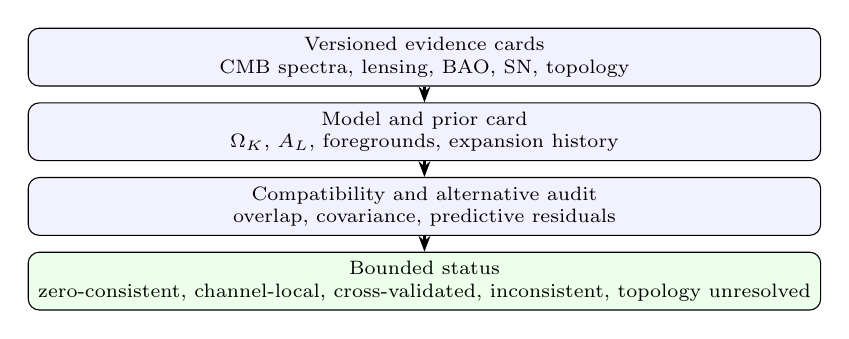
\begin{tikzpicture}[
  box/.style={draw, rounded corners, align=center, minimum width=0.83\columnwidth, minimum height=0.66cm, fill=blue!5, font=\scriptsize},
  decision/.style={draw, rounded corners, align=center, minimum width=0.83\columnwidth, minimum height=0.72cm, fill=green!8, font=\scriptsize},
  arrow/.style={-{Stealth[length=2mm]}, thick}
]
\node[box] (cards) {Versioned evidence cards\\CMB spectra, lensing, BAO, SN, topology};
\node[box, below=2mm of cards] (model) {Model and prior card\\$\ok$, $A_L$, foregrounds, expansion history};
\node[box, below=2mm of model] (audit) {Compatibility and alternative audit\\overlap, covariance, predictive residuals};
\node[decision, below=2mm of audit] (status) {Bounded status\\zero-consistent, channel-local, cross-validated, inconsistent, topology unresolved};
\draw[arrow] (cards) -- (model);
\draw[arrow] (model) -- (audit);
\draw[arrow] (audit) -- (status);
\end{tikzpicture}
\caption{\curvledger\ chain of custody. A conclusion may only move downward when its data-overlap, translation, and alternative-explanation conditions are recorded.}
\label{fig:ledger}
\end{figure}

\subsection{Chain of custody}

Figure~\ref{fig:ledger} maps a result from source to decision. A versioned evidence card records the release, measured object, likelihood, nuisance parameters, selection/mask, covariance statement, and permitted conclusion. A model card then specifies the cosmological parameter vector and priors. An audit card states whether likelihood multiplication is justified and which alternative mechanisms can produce similar residuals. Finally, a decision card uses fixed labels rather than a free-form declaration of discovery.

This architecture distinguishes evidence strength from conclusion breadth. A high signal-to-noise CMB spectrum can give a precise conditional $\ok$ posterior but still be unable to identify whether a peak-smoothing residual originates in curvature, phenomenological $A_L$, foreground treatment, or a more general model mismatch. A less precise but differently systematic BAO or independent-CMB card can then be decisive for attribution, not because it is ``more precise,'' but because it changes the error geometry.

\section{Design-Only Methods}

\subsection{Experimental unit and release manifest}

The computational experimental unit is a versioned \emph{likelihood-model card}, not a CMB pixel, individual galaxy, or published posterior plot. This avoids pseudo-replication. For example, Planck primary spectra and Planck lensing reconstruction are complementary but share sky and calibration dependencies; they cannot automatically be multiplied as independent experiments. Likewise, overlapping BAO releases are alternative cards unless a joint covariance model is supplied.

The frozen data manifest will contain six families. C1 is the Planck 2018 primary TT/TE/EE and low-multipole likelihood. C2 is the Planck lensing reconstruction. C3 is ACT DR6 spectra and, where suitable, lensing products. C4 is SPT-3G lensing. C5 contains non-overlapping eBOSS and DESI BAO release cards. C6 is an optional low-redshift validation family for supernovae and weak lensing. Each entry must include public release identifier, software/likelihood version, masks and multipole cuts, calibration and foreground specification, allowed parameter ranges, and a statement of shared information.

The design does not download or analyze any of these products. Its output is a preregistered protocol that a qualified cosmology analysis team can implement under the relevant data-use terms. The separation is important: an analysis plan can say exactly what would falsify a claim without pretending that it has observed the relevant result.

\subsection{Model ladder}

Table~\ref{tab:ladder} fixes the central model comparisons. The ladder is deliberately small enough to be interpretable and broad enough to challenge an anomaly-to-curvature interpretation. It does not attempt an unconstrained search over all new physics. Every extension has to declare how it alters the CMB, distance, and growth observables before it is used as an alternative.

\begin{table*}[t]
\caption{Predeclared \curvledger\ model ladder. No model is privileged because it fits one channel in isolation.}
\label{tab:ladder}
\centering
\footnotesize
\setlength{\tabcolsep}{3pt}
\begin{tabular}{L{0.10\textwidth}L{0.22\textwidth}L{0.28\textwidth}L{0.28\textwidth}}
\toprule
\textbf{Card} & \textbf{Parameter change} & \textbf{Primary scientific question} & \textbf{Required diagnostic}\\
\midrule
M0 & Flat \lcdm, $\ok=0$. & Does the baseline describe each card's observable? & Per-card posterior predictive residuals.\\
M1 & Non-flat \lcdm, free $\ok$. & Is a curvature degree of freedom demanded by a named card? & Prior sensitivity and CMB-to-BAO predictive transport.\\
M2 & M1 plus free phenomenological $A_L$. & Is peak smoothing being attributed uniquely to geometry? & Lensing-reconstruction comparison; forbid $A_L$ as physical curvature.\\
M3 & M1 plus predeclared foreground/calibration or primordial-spectrum robustness variants. & Does a curvature preference survive plausible likelihood alternatives? & Leave-one-variant-out stability and blinded injection recovery.\\
M4 & M1 plus a declared late-time expansion extension. & Can altered $E(z)$ reconcile CMB and distance data without curvature? & BAO/SN prediction and complexity-aware model comparison.\\
\bottomrule
\end{tabular}
\end{table*}

The parameter vector for a model card is $\theta_{\model}=\{\omega_b,\omega_c,\theta_s,\tau,A_s,n_s,\ok,\xi_{\model}\}$, where $\xi_{\model}$ contains only the extension parameters authorized by that card. Channel-specific nuisance parameters are denoted $\eta_c$. The intended posterior factorization is
\begin{align}
p(\theta_{\model},\{\eta_c\}\mid D,\model)
&\propto p(\theta_{\model}\mid\model)\prod_c \mathcal{L}_c(D_c\mid\theta_{\model},\eta_c,\model) \nonumber\\
&\quad\times p(\eta_c\mid\model).
\label{eq:posterior}
\end{align}
Equation~\eqref{eq:posterior} is used only after the compatibility audit determines that the product is admissible. If cards overlap without a valid joint covariance or likelihood, the product is prohibited. The cards must instead be compared through predictive checks or a correctly modeled joint analysis.

\subsection{Inference and compatibility protocol}

The implementation sequence is as follows. First, freeze the data and model cards before any sampling. Second, run channel-local inference for M0--M4 with convergence requirements declared in advance. Third, calculate posterior-predictive diagnostics in observable space: CMB spectra, lensing spectra, BAO distance combinations, or supernova residuals as appropriate. Fourth, document data overlap and external-prior reuse before combining cards. Fifth, evaluate only admissible joint combinations. Sixth, challenge any curvature preference using the alternative ladder and leave-one-card-out tests.

The compatibility question is not whether two posterior means agree by eye. For datasets $D_i$ and $D_j$, the proposed diagnostic suite includes predictive transport: infer $\theta_{\model}$ from $D_i$, predict a summary for $D_j$, and compare the residual to the released covariance and nuisance model. A tension is therefore a property of a named $(D_i,D_j,\model)$ triple, not a free-floating fact about the universe. A model that uses curvature to fit C1 but predicts implausible BAO distances in C5 is not evidence for a closed universe; it is a failed joint explanation.

\subsection{Robustness and false-positive controls}

Five stress tests provide a concrete falsification protocol. A prior ablation repeats M1 with defensible alternative $\ok$ prior ranges and parameterizations. A lensing ablation separates peak-smoothing information from reconstructed lensing. An instrument ablation withholds Planck, ACT, or SPT cards in turn. A low-redshift ablation withholds BAO release groups and supernova compilations separately. Finally, synthetic injection tests use simulated likelihood summaries generated under flat, closed, and nuisance-shift scenarios to estimate whether the decision taxonomy can falsely issue a cross-validated closed label.

The synthetic tests have a sharply defined failure mode. If a flat generator plus a calibration or $A_L$-like shift is regularly labeled `CLOSED\_PREFERENCE\_CROSS\_VALIDATED', the design is unsafe for discovery-level inference. If a closed generator cannot be distinguished from the alternatives at the planned sensitivity, the correct output is sensitivity-limited or model/likelihood inconsistent, not a null claim about reality.

\subsection{Pre-registered evaluation metrics and stopping conditions}

The study will not judge model cards using only a one-dimensional credible interval for $\ok$. Every card must generate four classes of prespecified diagnostics. The first is sampling and numerical validity: independent chains, convergence statistics, effective sample size, likelihood evaluations, and reproducible random seeds must meet thresholds chosen before unblinding. The second is within-channel fit: binned or otherwise released CMB, lensing, BAO, and supernova residuals must be evaluated against the stated covariance rather than summarized by a best-fit parameter alone. The third is cross-channel predictive transport: a posterior inferred from one evidence family must predict the held-out family with its own nuisance and calibration uncertainty. The fourth is robustness: the categorical CurvLedger output must remain stable, or its instability must be reported, under the ablations in the preceding subsection.

For a compact, auditable comparison, let $\mu_i$ and $\Sigma_i$ denote an agreed parameter-summary mean and covariance for a named card $i$. A diagnostic distance may be defined as
\begin{equation}
\Delta_{ij}^2=(\mu_i-\mu_j)^T(\Sigma_i+\Sigma_j)^{-1}(\mu_i-\mu_j),
\label{eq:distance-diagnostic}
\end{equation}
only when the summaries share a parameterization and the covariance sum is justified. Equation~\eqref{eq:distance-diagnostic} is not a replacement for a joint likelihood, and it must not be used where shared data invalidate the independence approximation. Its role is triage: a large value triggers a posterior-predictive and overlap audit; it never independently diagnoses curvature.

Table~\ref{tab:metrics} specifies the stopping conditions. A failure at any upstream condition prevents promotion to a broader scientific label. For example, a sampler can converge perfectly on an incomplete foreground model; numerical convergence then certifies only the computation, not the model. Likewise, a statistically sharp CMB-only negative-$\ok$ interval cannot advance if the relevant lensing or BAO cards reject the forward prediction. This is the key distinction between precision and identification.

\begin{table}[t]
\caption{Pre-registered metrics and stopping rules.}
\label{tab:metrics}
\centering
\scriptsize
\setlength{\tabcolsep}{2.2pt}
\begin{tabular}{L{0.27\columnwidth}L{0.35\columnwidth}L{0.28\columnwidth}}
\toprule
\textbf{Metric} & \textbf{Pass condition} & \textbf{Failure action}\\
\midrule
Numerical validity & Frozen code/version, convergence and effective sample-size thresholds passed. & Do not interpret any posterior.\\
Likelihood fidelity & Released nuisance model and covariance retained; residual checks pass. & Flag likelihood-local result.\\
Cross-probe transport & Held-out observable prediction is compatible after declared overlap treatment. & Issue inconsistency, not a combined constraint.\\
Alternative challenge & M2--M4 do not explain the residual equally well or better. & Retain channel-local / alternative-degenerate label.\\
Topology guard & A topology likelihood exists and is independently reviewed. & Keep topology unresolved.\\
\bottomrule
\end{tabular}
\end{table}

\subsection{Reproducibility package and decision ledger}

A completed implementation would publish more than a final contour. The reproducibility package must contain a machine-readable data manifest; exact likelihood versions; model equations and prior bounds; covariance and overlap decisions; nuisance parameter definitions; sampler settings; convergence diagnostics; posterior-predictive outputs; and a decision ledger recording why a label was assigned. A ledger entry should link a label to the evidence cards that support it, the cards withheld, the alternative cards tested, and the reviewer responsible for the covariance decision. This design makes negative findings scientifically useful: a robust `MODEL OR LIKELIHOOD INCONSISTENT' status identifies which prediction fails and which next measurement could resolve it.

A blinded-analysis rule applies whenever a collaborating release supports it. Analysis choices, robustness variants, and status thresholds must be registered before inspecting the final curvature posterior. Post-unblinding changes must be logged, motivated, and rerun from the frozen baseline. This is particularly important because the research question has a salient expected answer---flat versus closed---and therefore is unusually exposed to subtle confirmation bias in prior choice, multipole cut, or data-combination selection.
\section{Observable Matrix and Decision Logic}

Table~\ref{tab:matrix} connects the relevant physical mechanisms to their observables and alternatives. It is not a forecast of a measured constraint. Its purpose is to prevent an analysis from treating a residual in one column as a unique signature of the mechanism in the first column.

\begin{table*}[t]
\caption{Curvature-observable matrix. ``Discriminator'' means a planned measurement or test that can distinguish, not an already achieved result.}
\label{tab:matrix}
\centering
\footnotesize
\setlength{\tabcolsep}{3pt}
\begin{tabular}{L{0.20\textwidth}L{0.23\textwidth}L{0.25\textwidth}L{0.22\textwidth}}
\toprule
\textbf{Mechanism card} & \textbf{Relevant observables} & \textbf{Confusable alternatives} & \textbf{Required discriminator}\\
\midrule
Nonzero spatial curvature & Acoustic-scale distance, CMB peak pattern, BAO transverse/radial distance, SN distance relation. & Dark-energy history, sound-horizon changes, prior volume. & Joint predictive transport from CMB to BAO/SN under the same forward model.\\
Peak-smoothing anomaly & High-$\ell$ TT/TE/EE smoothing. & Free $A_L$, foreground template, beam/calibration, primordial feature. & Compare to lensing reconstruction and independent ACT/SPT spectra.\\
Late-time expansion extension & $D_M(z)$, $H(z)$, SN distances, structure growth. & Curvature-distance degeneracy, supernova calibration, BAO covariance. & Separate M4 posterior-predictive checks with release-level nuisance cards.\\
Nontrivial topology & Matched patterns/circles or topology-specific CMB correlations. & Mask, foreground, chance alignment, transfer-function model. & Registered topology likelihood independent of the $\ok$ posterior.\\
\bottomrule
\end{tabular}
\end{table*}

\subsection{Fixed status taxonomy}

The final taxonomy is shown in Table~\ref{tab:status}. The labels are intentionally conservative about conclusion breadth but direct about what a specific analysis demonstrates. A status is neither a Bayesian model probability detached from its priors nor a journal-style claim. It is an audit outcome that tells a reader where the evidence survives and where it does not.

\begin{table}[t]
\caption{Fixed outputs for the planned curvature study.}
\label{tab:status}
\centering
\scriptsize
\setlength{\tabcolsep}{2.5pt}
\begin{tabular}{L{0.37\columnwidth}L{0.53\columnwidth}}
\toprule
\textbf{Output} & \textbf{Meaning}\\
\midrule
CURVATURE CONSISTENT WITH ZERO & The declared model and compatible cards do not demand $\ok\ne0$.\\
CLOSED PREFERENCE CHANNEL LOCAL & A named card/model favors $\ok<0$ but has not passed replication and alternative tests.\\
CLOSED PREFERENCE CROSS VALIDATED & Compatible independent cards support an overlapping closed region and alternatives fail the predeclared tests.\\
MODEL OR LIKELIHOOD INCONSISTENT & No common model region predicts all included cards; this is not curvature evidence by itself.\\
TOPOLOGY UNRESOLVED & No topology-specific observable has been tested successfully.\\
\bottomrule
\end{tabular}
\end{table}

The central decision rule is therefore conditional. Suppose M1 produces a negative-$\ok$ posterior from Planck C1. The output may be `CLOSED PREFERENCE CHANNEL LOCAL' only if the exact C1 likelihood, priors, and posterior-predictive behavior are recorded. The label can advance only if an independent CMB or lensing card passes a compatibility audit, the predicted BAO/SN quantities are acceptable, and M2--M4 fail to account for the effect without curvature. If any of these requirements is absent, the correct label is not a weakened discovery claim; it is an explicit limitation.

\section{Falsification, Identifiability, and Human Review}

\subsection{What could change the conclusion?}

The design is falsifiable in both directions. A cross-validated closed result would be undermined by an independently calibrated CMB spectrum or lensing reconstruction that rejects the same parameter region, by BAO/SN predictive failure, or by a declared non-curvature alternative that predicts all channels better. Conversely, a present flat-compatible conclusion would be revised if future independent likelihoods produce a coherent closed region with a well-defined covariance treatment and no viable alternative explanation. In both cases, the target is a constrained model statement, not an absolute metaphysical verdict.

Identifiability is assessed at the level of forward maps. If two model cards yield indistinguishable predictions over the available observables, the design cannot declare one preferred merely because its posterior is narrow under a selected prior. It must report an observationally unresolved mechanism or collect another discriminator. This guard is especially important for the relationship between $\ok$ and $A_L$: the latter is a phenomenological scaling used to describe spectrum smoothing, not a physical measurement of spatial curvature.

\subsection{Human review requirements}

The workflow requires qualified human review at four points. A CMB-likelihood expert must approve high-$\ell$ foreground, beam, calibration, and multipole-cut handling. A statistics reviewer must approve dataset-overlap and covariance treatment before any product likelihood is used. A data steward must verify release licences, software versions, and blinding rules. A cosmology interpretation reviewer must inspect whether the final prose preserves the difference between a posterior result, an anomaly, a curvature model, and topology. These reviews are scientific controls, not generic disclaimers: they target the exact ways a false curvature claim could be produced.

\section{Expected Outcome Branches and Conditional Interpretation}

The proposed study is designed to make a conclusion conditional on observable behavior rather than on the attractiveness of an answer. Table~\ref{tab:branches} enumerates the major branches before data analysis. Each branch has a different scientific interpretation and a different next experiment. This is preferable to an after-the-fact narrative in which every residual is treated as support for the preferred hypothesis.

\begin{table*}[t]
\caption{Predeclared outcome branches. The entries describe decision logic, not results from this proposal.}
\label{tab:branches}
\centering
\footnotesize
\setlength{\tabcolsep}{3pt}
\begin{tabular}{L{0.22\textwidth}L{0.31\textwidth}L{0.35\textwidth}}
\toprule
\textbf{Observed pattern after a future implementation} & \textbf{CurvLedger classification} & \textbf{Scientific interpretation and next action}\\
\midrule
All compatible CMB, lensing, BAO, and SN cards admit $\ok=0$; no structured residual remains. & CURVATURE CONSISTENT WITH ZERO & Flat FLRW remains an adequate description in the tested model space. Extend precision only where it adds a distinct systematic response; do not infer topology or infinity.\\
A negative-$\ok$ region appears only in a Planck primary-spectrum card or disappears when $A_L$ / nuisance alternatives are released. & CLOSED PREFERENCE CHANNEL LOCAL & Diagnose spectrum-level smoothing, foreground, calibration, and likelihood sensitivity. Obtain independent polarization and lensing discriminators before any geometric claim.\\
Independent CMB/lensing cards and low-redshift geometry support the same closed region; alternatives fail predictive tests. & CLOSED PREFERENCE CROSS VALIDATED & Report a model-bounded curvature preference with priors, covariance, and failed alternatives. Start a separate topology program rather than inferring topology.\\
No single parameter region predicts the included cards under a declared model, even after allowed extensions. & MODEL OR LIKELIHOOD INCONSISTENT & Localize the failed forward prediction, test covariance and systematics, and enlarge the model only through a predeclared physical mechanism. Do not label the tension curvature.\\
A topology-specific observable is absent or non-diagnostic. & TOPOLOGY UNRESOLVED & State explicitly that neither flatness nor closure has settled global identifications, total volume, or return paths.\\
\bottomrule
\end{tabular}
\end{table*}

\subsection{Branch A: a stable flat-compatible geometry}

A future flat-compatible result is not a null outcome in the colloquial sense. It would show that, across the declared model ladder and compatible evidence cards, there is no requirement for a curvature parameter beyond zero. The result would be stronger than a CMB-only interval because it would include predictive transport to late-time distances and independent CMB observables. It would still not prove that the universe is infinite. Compact flat topologies are a separate family of models, and finite observational reach prevents a direct survey of the entire spatial slice.

The relevant next action in this branch is targeted precision: improve polarization, lensing reconstruction, BAO calibration, and supernova control only to the extent that these measurements create new discriminating directions. Repeating a highly correlated summary statistic with smaller error bars may narrow a posterior without increasing identifiability. The ledger makes that distinction measurable through the shared-information and held-out-prediction fields.

\subsection{Branch B: a channel-local closed preference}

A channel-local closed preference is also a meaningful outcome, provided it is described accurately. It identifies a feature in a named likelihood/model card that is not yet explained by the baseline. The correct response is to inspect the observable-level residual, test the M2--M4 alternatives, and seek independent data with different beams, frequency coverage, sky masks, calibration chains, or redshift response. The response is not to average the feature away, nor to call it a measurement of global closure.

This branch directly addresses the historical Planck situation. The Planck spectra, lensing reconstruction, BAO combinations, and later independent CMB products should be treated as a structured diagnostic network. A disagreement can teach cosmology about foreground modeling, lensing reconstruction, primordial physics, or late-time expansion even if the eventual curvature posterior is consistent with zero. The study therefore preserves anomaly information instead of forcing every source into a premature consensus.

\subsection{Branches C and D: replicated curvature or model failure}

A cross-validated closed result would require the strictest threshold. The common closed region must survive a declared curvature convention and prior family, pass independent-instrument replication, correctly predict BAO/SN distances, and resist the specified non-curvature alternatives. This would justify a direct statement about spatial curvature within a named model family. It would not answer all versions of the shape question: neither topology nor the physical origin of the curvature parameter follows automatically.

Alternatively, persistent incompatibility can be the scientifically decisive outcome. If no M0--M4 card predicts all selected observables after covariance review, the proposal calls for a model-or-likelihood inconsistency label. This outcome is valuable because it keeps the cause localized. It identifies which prediction fails, which nuisance or physical extensions were tested, and which measurement most efficiently distinguishes the remaining explanations. Such an outcome prevents a broad cosmological crisis from becoming an untestable slogan.
\section{Discussion: From a Shape Question to a Testable Program}

The phrase ``the universe is flat'' is often shorthand for an extremely successful standard cosmological description, not a proof that space is globally Euclidean, infinite, or topologically trivial. Likewise, a Planck-only closed posterior is not empty information. It identifies a structured stress test involving CMB peak smoothing, lensing inference, and the geometric degeneracies that BAO and other probes can break. The scientific error is not considering the closed interpretation; it is treating a conditional preference as a universal conclusion before it survives the tests that its own model makes possible.

\curvledger\ makes those tests legible. It replaces an informal chain---``one dataset prefers closure, another prefers flatness''---with a reproducible sequence: state the observable, freeze the likelihood and priors, transport the model to another probe, account for shared information, challenge alternatives, and issue a bounded status. This is applicable beyond curvature. The same structure can be used for lensing anomalies, primordial-spectrum features, neutrino-mass inferences, or modified-gravity claims where a precise measurement in one channel is not automatically a unique physical identification.

The design also clarifies the place of future surveys. Improved polarization, high-resolution CMB lensing, independently calibrated BAO, and expanded weak-lensing samples are valuable insofar as they add genuinely distinct response kernels and systematic controls. The Simons Observatory science program illustrates why richer multifrequency CMB measurements can improve both parameter precision and foreground/lensing discrimination~\cite{simons19}. Their value for the present question is not simply smaller error bars on $\ok$; it is the ability to test whether the same physical model predicts several observables at once.

\section{Conditional Conclusions}

This four-agent proposal answers the initial question in a form that observations can adjudicate. Present evidence supports three statements. First, spatial curvature is a model-dependent parameter inferred from a network of distances and spectra, not an image of the universe viewed from outside. Second, Planck's published closed-curvature interpretation is scientifically relevant but conditional and entangled with a lensing-like smoothing anomaly; it cannot be promoted to a consensus global shape claim when other declared probe combinations are consistent with flatness~\cite{planck18,act25,eboss21}. Third, curvature and topology remain separate: even a future robust curvature result would not by itself establish whether space is finite or multiply connected.

The resulting experimental program is direct. If an overlapping negative-$\ok$ region survives independent CMB/lensing replication, BAO/SN predictive transport, covariance review, and the M2--M4 alternative challenge, the proper conclusion is a model-bounded cross-validated closed preference. If the signal remains tied to one Planck likelihood configuration or disappears under an alternative treatment, the correct conclusion is channel-local or model/likelihood inconsistent. If no topology-specific likelihood is run, topology stays unresolved. These branches turn a broad cosmological question into a transparent set of falsifiable outcomes without claiming that any new measurement has already been made.

\IEEEtriggeratref{5}
\begin{thebibliography}{00}
\bibitem{planck18} Planck Collaboration, ``Planck 2018 results. VI. Cosmological parameters,'' \emph{Astronomy \& Astrophysics}, vol. 641, A6, 2020, doi: 10.1051/0004-6361/201833910.
\bibitem{dival19} E. Di Valentino, A. Melchiorri, and J. Silk, ``Planck evidence for a closed Universe and a possible crisis for cosmology,'' \emph{Nature Astronomy}, vol. 4, pp. 196--203, 2020, doi: 10.1038/s41550-019-0906-9.
\bibitem{dival20} E. Di Valentino, A. Melchiorri, and J. Silk, ``Cosmological constraints in extended parameter space from the Planck 2018 Legacy release,'' \emph{Journal of Cosmology and Astroparticle Physics}, vol. 2020, no. 01, 013, 2020, doi: 10.1088/1475-7516/2020/01/013.
\bibitem{eboss21} S. Alam \emph{et al.}, ``Completed SDSS-IV extended Baryon Oscillation Spectroscopic Survey: Cosmological implications from two decades of spectroscopic surveys,'' \emph{Physical Review D}, vol. 103, 083533, 2021, doi: 10.1103/PhysRevD.103.083533.
\bibitem{spt23} Z. Pan \emph{et al.}, ``Measurement of gravitational lensing of the cosmic microwave background using SPT-3G 2018 data,'' \emph{Physical Review D}, vol. 108, 122005, 2023, doi: 10.1103/PhysRevD.108.122005.
\bibitem{desi25} A. G. Adame \emph{et al.}, ``DESI 2024 VI: cosmological constraints from the measurements of baryon acoustic oscillations,'' \emph{Journal of Cosmology and Astroparticle Physics}, vol. 2025, no. 02, 021, 2025, doi: 10.1088/1475-7516/2025/02/021.
\bibitem{act25} T. Louis \emph{et al.}, ``The Atacama Cosmology Telescope: DR6 power spectra, likelihoods and $\Lambda$CDM parameters,'' \emph{Journal of Cosmology and Astroparticle Physics}, vol. 2025, no. 11, 062, 2025, doi: 10.1088/1475-7516/2025/11/062.
\bibitem{simons19} P. A. R. Ade \emph{et al.}, ``The Simons Observatory: science goals and forecasts,'' \emph{Journal of Cosmology and Astroparticle Physics}, vol. 2019, no. 02, 056, 2019, doi: 10.1088/1475-7516/2019/02/056.
\end{thebibliography}

\end{document}
